\chapter[]{Roslyn Compiler Call Chain}
In \bsref{fig:roslyn_invoke_overview} an overview of the compilation call chain is shown. A compilation starts with \bscode{csc}'s main method being invoked, which calls the static \bscode{Run} method on the \bscode{Csc} class. This method creates a new \bscode{compiler} object of type \bscode{Csc}. \bscode{Csc} is a subtype of \bscode{CSharpCompiler}, located in the \bscode{CSharp.CSharpCodeAnalysis.Desktop} project, which again is a subtype of \bscode{CommonCompiler}, located in \bscode{Core.CodeAnalysis}. This means that the creation of the \bscode{compiler} object, calls the constructors of \bscode{Csc}, \bscode{CSharpCompiler} and \bscode{CommonCompiler}. Afterwards the \bscode{Run} method is invoked on the \bscode{compiler} object, which further invokes its parent's \bscode{Run} method, which again invokes its parent's \bscode{Run} method. Finally the \bscode{RunCore} method in \bscode{CommonCompiler} is invoked, which contains the general code that controls the overall flow of the compiler pipeline, illustrated in \bsref{fig:api_vs_compiler_pipeline}. The \bscode{RunCore} method will, for each phase, call the language specific implementation of the phase, located in either C\# in \bscode{CSharp.CSharpCodeAnalysis.Portable} or \ac{VB} in \bscode{VisualBasic.BasicCodeAnalysis.Portable}, through dynamic dispatch.
\label{app:roslyn_call_chain}
\begin{sidewaysfigure}[htbp]
\centering
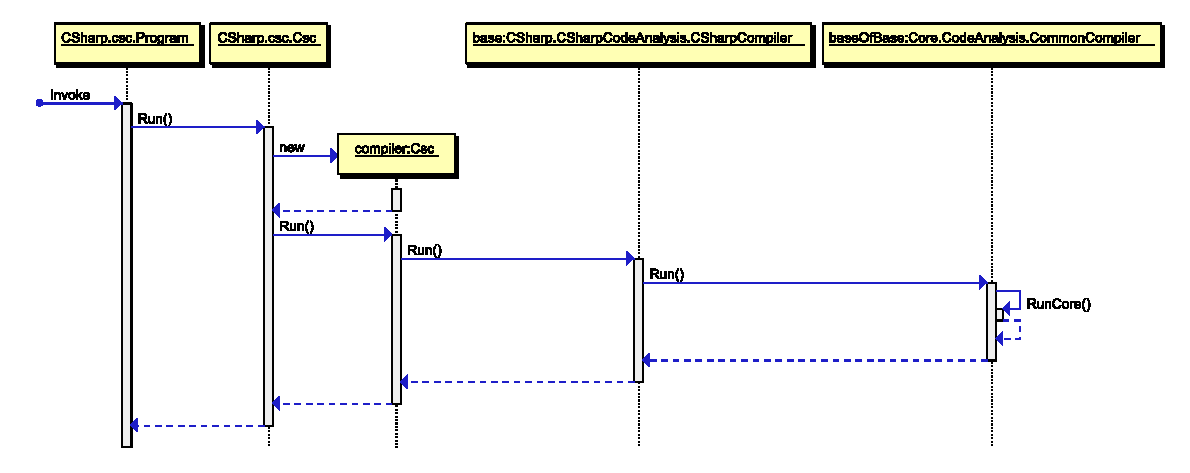
\includegraphics[width=\textwidth]{\rootpath/worksheets/appendix/figures/seq_diagrams/roslyn_invoke_overview}
\caption{Sequence diagram showing an overview of the call chain of a C\# compilation.}
\label{fig:roslyn_invoke_overview}
\end{sidewaysfigure}
